\documentclass{article}
\usepackage{amsmath}
\usepackage{amssymb}
\usepackage{amsthm}
\usepackage{graphicx}
\usepackage[margin=1.0in]{geometry}
\usepackage{fancyhdr} % for headers and footers
\usepackage[nobreak=false]{mdframed}
\usepackage{bm} %vectors
\usepackage[dvipsnames]{xcolor}
\usepackage{multicol}
\usepackage{caption}
\usepackage{enumitem}
\usepackage{comment}
\usepackage{hyperref}
\newenvironment{greytext}{\color{Gray}}{\ignorespacesafterend}

\newcommand{\volume}{\mathop{\ooalign{\hfil$V$\hfil\cr\kern0.08em--\hfil\cr}}\nolimits} % Fluid dynamics volume

\newcommand{\fixthis}[1]{} %comment to see if you still have things to do



\pagestyle{fancy}
\lhead{Valmik Prabhu}
\rhead{Axle Installation Guide} % FILL THIS IN!
\cfoot{} % stops default numbering
\rfoot{Page~\thepage}

\title{B17 Axle Installation Guide}
\author{Valmik Prabhu}

\begin{document}

\parindent = 0pt

\maketitle

\section{Check the Differential Assembly}
The diff must be installed properly before axles can be installed. First make sure that the diff is mounted properly. All four bolts must be installed and at least hand-tight. They do not need to be torqued, but torquing is probably easier without axles in the way.

\begin{minipage}{\linewidth}
$\,$

\begin{center}
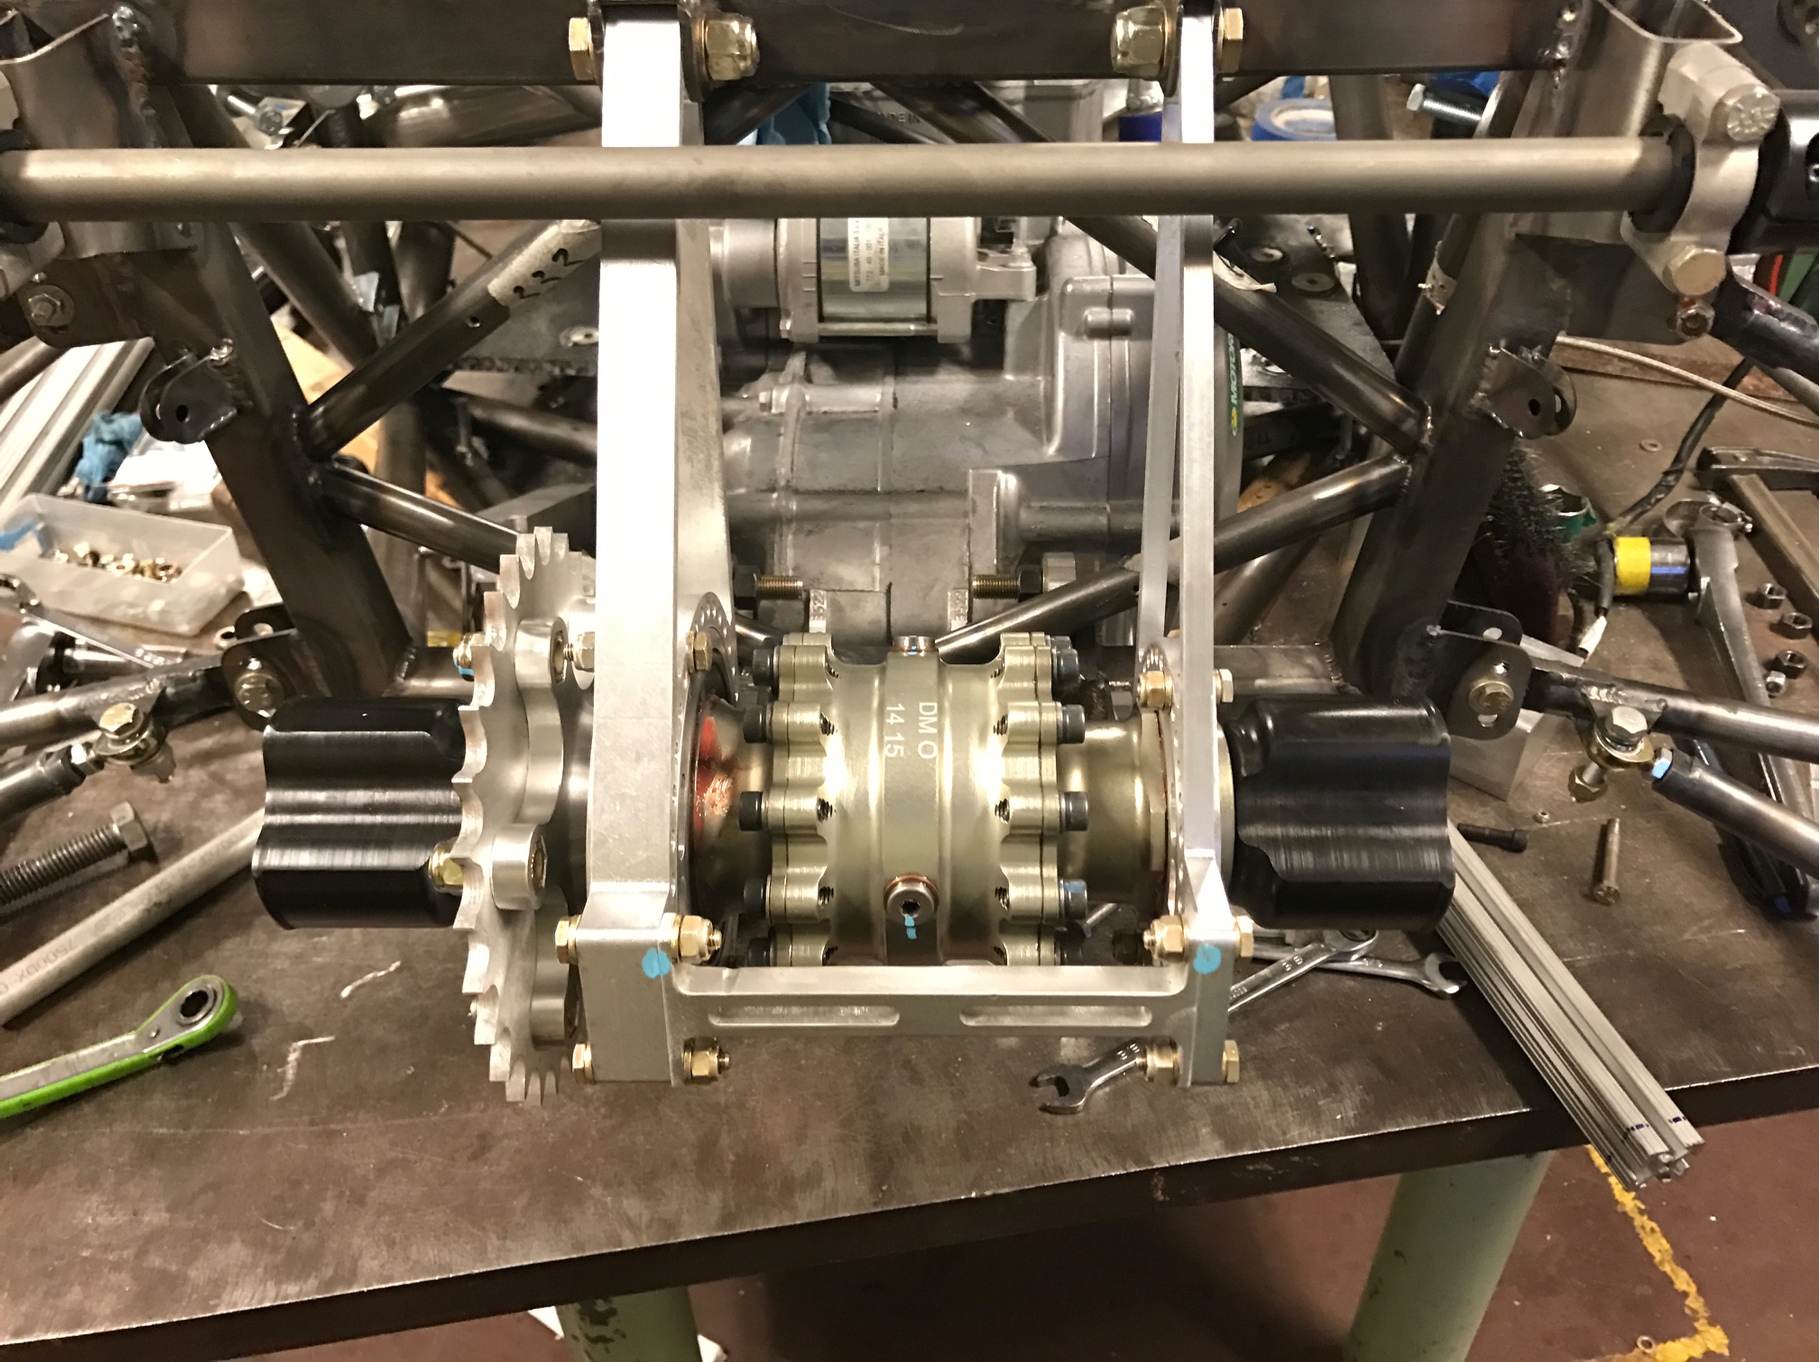
\includegraphics[width = 150pt]{Diff.png}

\captionof{figure}{This is what the diff looks like when installed}
\end{center}
$\,$
\end{minipage}

In addition, the inboard housings must be bolted into the diff and torqued. THESE BOLTS ARE INACCESSIBLE when axles are mounted and MUST BE TORQUED FIRST. These bolts are torqued with a special alan extension in the DT diff box. If you don't know how to install these bolts, please ask a DT member. If installed wrong, they can potentially bone the diff.

\begin{minipage}{\linewidth}
$\,$

\begin{center}
\includegraphics[width = 150pt]{InboardHousing.png}

\captionof{figure}{Make sure there's a torqued bolt inside each of these}
\end{center}
$\,$
\end{minipage}


\section{Check the Axles}

The axles should already be assembled, but you should check to make sure they're assembled properly. First check that there's one of each kind of boot on each axle. One boot has a triangular interior meant to fit the inboard housing, while the other has a circular interior meant to fit the outboard housing.

\begin{minipage}{\linewidth}
$\,$

\begin{center}
\includegraphics[width = 150pt]{Axle.png}

\captionof{figure}{The left boot is for the outboard housing, and the right one is for the inboard housing}
\end{center}
$\,$
\end{minipage}

Make sure that each side of the axle has a tripod mounted to it, and that each tripod is retained by two snap rings. Make sure the snap rings are tight and securely mounted. If a snap ring fails during a run, our car dies. If you don't trust one of the snap rings, please replace it from the 2017 Axles box in the DT tote or shelf.

\begin{minipage}{\linewidth}
$\,$

\begin{center}
\includegraphics[width = 150pt]{TripodZoom.png}

\captionof{figure}{Note the snap ring on each side of the tripod}
\end{center}
$\,$
\end{minipage}

\section{Check the Suspension}

The suspension arms should already be on the car and secured well. They don't need to be torqued, but they need to be secure enough to support the wheel packages.

\begin{minipage}{\linewidth}
$\,$

\begin{center}
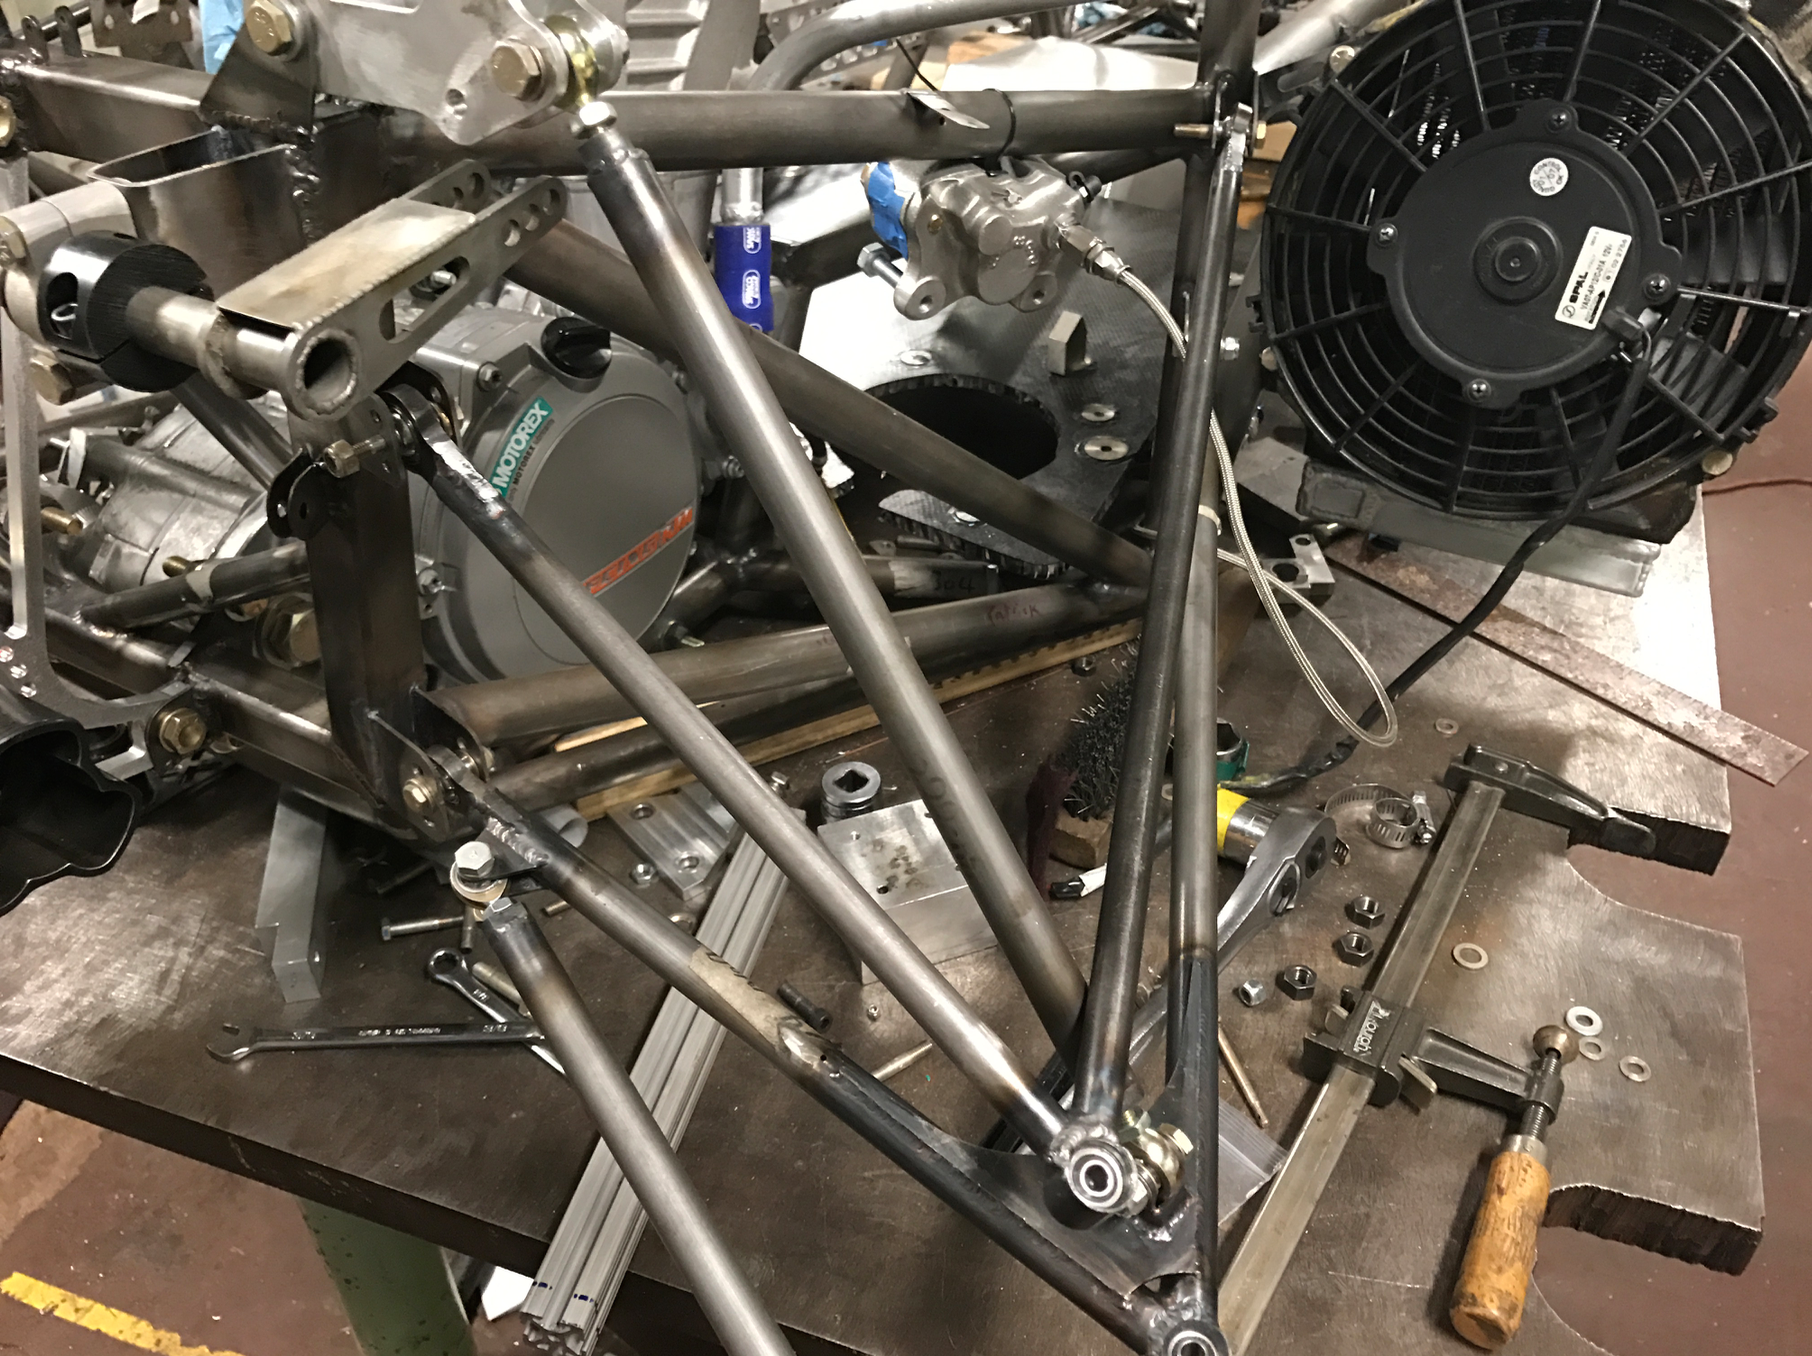
\includegraphics[width = 150pt]{Suspension.png}

\captionof{figure}{All four suspension arms should be mounted}
\end{center}
$\,$
\end{minipage}

\section{Check the Rear Wheel Package}

The wheel package axially retains the axles. First, make sure that the package is pressed together properly. Primarily, check that the wheel speed sensor disk is on and undamaged, both bearing shields are on, there's no axial slop on the components, and the upright spins freely.

\begin{minipage}{\linewidth}
$\,$

\begin{center}
\includegraphics[width = 150pt]{WheelPackage.png}

\captionof{figure}{This is the rear wheel package}
\end{center}
$\,$
\end{minipage}

Next, make sure that the outboard housing is properly bolted to the package. While it doesn't have to be torqued (and probably shouldn't until it's on the car) it needs to be tight enough that the bolt head cannot slip out of the retaining feature on the outboard housing. The head is inaccessible while the axle is mounted, so if the head slips out of the retaining feature in the outboard housing while the axle is mounted, it's really easy to mess up something while tightening.

\begin{minipage}{\linewidth}
$\,$

\begin{center}
\includegraphics[width = 150pt]{OutboardBolt.png}

\captionof{figure}{Here's the bolt head inside the outboard housing}
\end{center}
$\,$
\end{minipage}

Lastly, you'll need to make sure that the insert and snap ring are in the housing. Make sure to inspect the insert for (new) cracks and check for wear around the snap ring groove or the base of the outboard housing.

\begin{minipage}{\linewidth}
$\,$

\begin{center}
\includegraphics[width = 150pt]{InsertPic.png}

\captionof{figure}{Here's the insert and snap ring}
\end{center}
$\,$
\end{minipage}


\section{Install the Axles}

Now you install everything. This is a two person job, so make sure you've got someone to help you. The first step is to remove the snap ring from the outboard housing. Use the snap ring pliers in the B17 Axle Box.

\begin{minipage}{\linewidth}
$\,$

\begin{center}
\includegraphics[width = 150pt]{SnapRingOut.png}

\captionof{figure}{Removed snap ring and pliers}
\end{center}
$\,$
\end{minipage}

Now insert the inboard tripod of the axle into the inboard housing (on the diff). Make sure you're inserting the correct side of the axle (the one with the three-lobe boot on it) into the outboard housing, or you'll have to redo everything later and it'll suck.

\begin{minipage}{\linewidth}
$\,$

\begin{center}
\includegraphics[width = 150pt]{AxleHalfIn.png}

\captionof{figure}{The axle in the inboard housing. One person will need to hold it like this until the upright is installed}
\end{center}
$\,$
\end{minipage}

Now pick up the wheel package, being careful to not let the insert slip out, and insert the outboard side of the axle into the outboard housing. At this point, you're essentially holding one side of the drive train in position.

\begin{minipage}{\linewidth}
$\,$

\begin{center}
\includegraphics[width = 150pt]{AxleHoldOn.png}

\captionof{figure}{Holding everything like this is why you need two people}
\end{center}
$\,$
\end{minipage}

Now mount the upright, making sure to not let any of the axle parts fall out of place. You need to mount the upper a arms, lower a arms and toe rods. One person can do this, while the other holds everything up.

Once the upright is installed, you need to reinstall the snap ring. Make sure the insert is all the way in, and the snap ring isn't worn.

\begin{minipage}{\linewidth}
$\,$

\begin{center}
\includegraphics[width = 150pt]{SnapRingInstall.png}

\captionof{figure}{Installing the snap ring}
\end{center}
$\,$
\end{minipage}

Now slide up the boots over each housing.

\begin{minipage}{\linewidth}
$\,$

\begin{center}
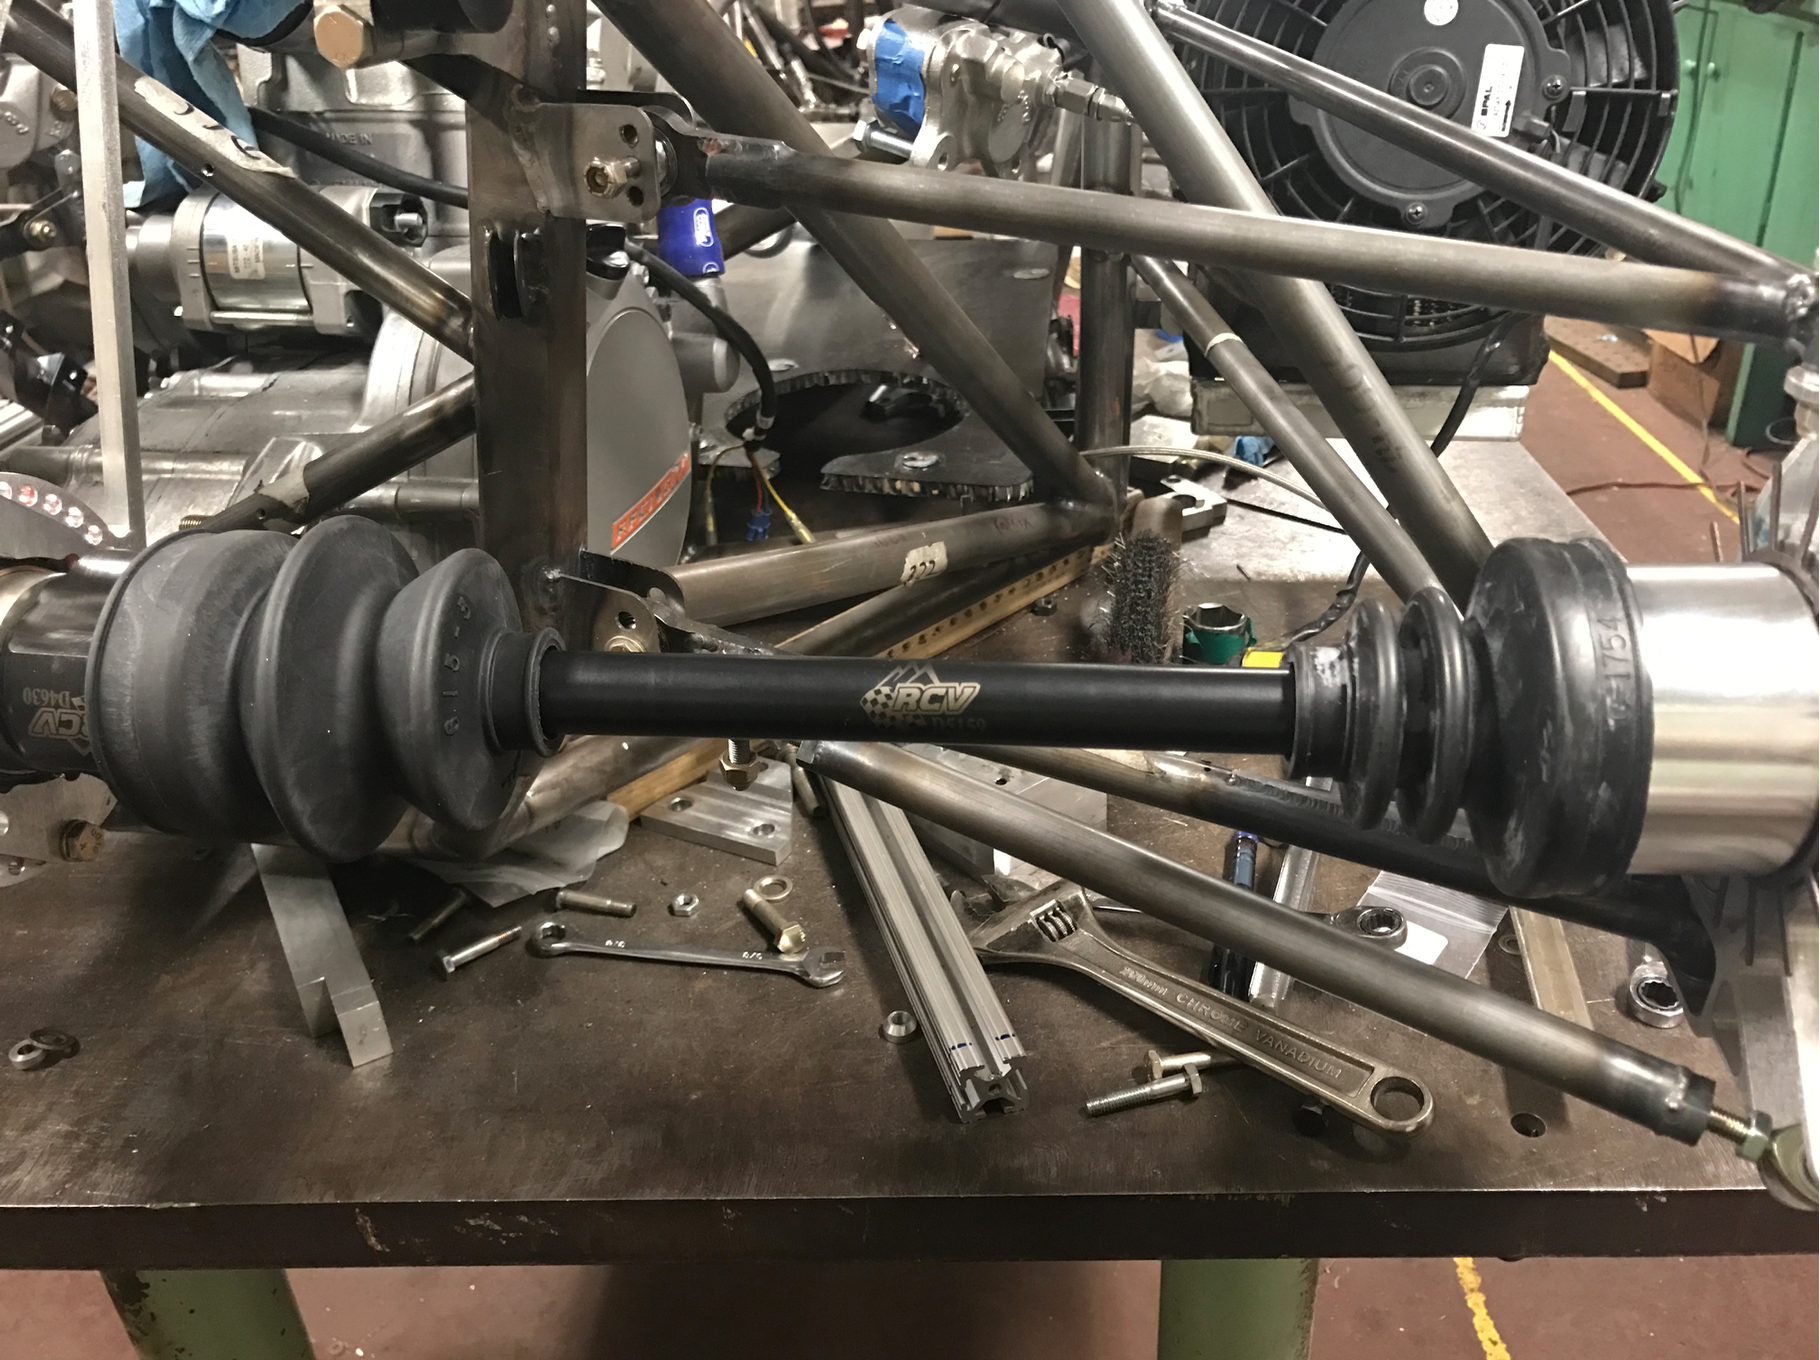
\includegraphics[width = 150pt]{AllDone.png}

\captionof{figure}{This is where you get screwed if you installed the axles backwards}
\end{center}
$\,$
\end{minipage}

And lastly top off the grease in each housing, and tighten the hose clamps over the boots. We haven't figured out how we're going to do this yet, so you can skip it for now.




% \section{Appendix: Code}

\begin{verbatim}

\end{verbatim}



%%%%%%%%%%%%%%%%%%%%%%%%%%%%%%%%%%% Code Snippets
\begin{comment}
Problem: *****************************
% ************************************** P1 *****************
\item \textbf{TITLE}

**************************************

Image: *******************************
\begin{minipage}{\linewidth}
\begin{center}
\includegraphics[width = 150pt]{IMAGE.png}

\captionof{figure}{CAPTION}
\end{center}
$\,$
\end{minipage}

**************************************

Solution: ****************************
\begin{mdframed}
\textbf{Solution: } \\ \fixthis{}

\end{mdframed}

**************************************

\end{comment}


\end{document}